% filepath: /home/sree/git/jax_bhm/doc/hierarchical_bayesian_modeling/bhm_notes_smc.tex
\documentclass[11pt,a4paper]{article}

% Packages
\usepackage{amsmath,amssymb,amsthm}
\usepackage{graphicx}
\usepackage{booktabs}
\usepackage{hyperref}
\usepackage{natbib}
\usepackage{algorithm}
\usepackage{algpseudocode}
\usepackage{tikz}
\usetikzlibrary{arrows,shapes,positioning,calc,fit}

% Formatting
\usepackage[margin=1in]{geometry}
\setlength{\parskip}{0.5em}
\setlength{\parindent}{0em}

% Custom commands
\newcommand{\btheta}{\boldsymbol{\theta}}
\newcommand{\bsigma}{\boldsymbol{\sigma}}
\newcommand{\btau}{\boldsymbol{\tau}}
\newcommand{\bx}{\mathbf{x}}
\newcommand{\by}{\mathbf{y}}
\newcommand{\bX}{\mathbf{X}}
\newcommand{\R}{\mathbb{R}}
\newcommand{\E}{\mathbb{E}}
\newcommand{\Var}{\mathrm{Var}}
\newcommand{\Normal}{\mathcal{N}}
\newcommand{\HalfCauchy}{\mathrm{HalfCauchy}}
\newcommand{\InvGamma}{\mathrm{InvGamma}}
\newcommand{\GammaDist}{\mathrm{Gamma}}
\newcommand{\Uniform}{\mathrm{Uniform}}

\theoremstyle{definition}
\newtheorem{definition}{Definition}
\newtheorem{remark}{Remark}

\title{Bayesian Hierarchical Modeling for Integrative Structural Biology:\\
\large Combining Cryo-EM, Cross-linking Mass Spectrometry, and Subunit Assembly Data\\[0.5em]
\normalsize With Applications to Heterogeneous Macromolecular Assemblies}

\author{JAX-BHM Documentation}
\date{\today}

\begin{document}

\maketitle

\begin{abstract}
We present a Bayesian hierarchical framework for integrating multiple experimental data sources in structural biology. Our approach combines three levels of information: (1) high-precision intra-tetramer distances from purified subunit experiments, (2) lower-precision inter-particle distances from cross-linking mass spectrometry (XL-MS), and (3) global shape information from cryo-electron microscopy (cryo-EM) density maps. We show how nuisance parameters (experimental uncertainties) at each level can be connected through hyperpriors, enabling principled uncertainty quantification and automatic calibration of relative data weights. Crucially, for intrinsically heterogeneous systems such as the postsynaptic density (PSD), we demonstrate that apparent ``noise'' in experimental data often reflects genuine biological variability rather than instrumental error. By introducing a latent hyperparameter governing \textit{systematic biological heterogeneity}, we statistically link uncertainties across diverse data sources, transforming data inconsistencies from obstacles into informative signals about the underlying conformational ensemble. Sequential Monte Carlo (SMC) sampling provides an efficient computational strategy for exploring the resulting posterior distribution.
\end{abstract}

\tableofcontents
\newpage

% ===========================================================================
\section{Introduction}
% ===========================================================================

Integrative structural biology combines multiple experimental data sources to determine the three-dimensional structures of macromolecular complexes. Each data source provides complementary information but comes with its own characteristic uncertainties and systematic errors.

The key challenge is: \textbf{how do we combine heterogeneous data in a principled way?}

Traditional approaches assign fixed weights to each data source based on intuition or trial-and-error. Bayesian hierarchical modeling offers a principled alternative where:
\begin{itemize}
    \item Experimental uncertainties are treated as \textit{nuisance parameters} to be inferred
    \item Related uncertainties are connected through \textit{hyperpriors}
    \item The data itself informs the relative weighting through \textit{posterior inference}
\end{itemize}

% ===========================================================================
\section{The Challenge of Biological Heterogeneity: Noise as Signal}
% ===========================================================================

\subsection{The Heterogeneity Paradox}

Many macromolecular assemblies---particularly large, dynamic complexes like the postsynaptic density (PSD), nuclear pore complex, or viral capsids---exhibit extreme structural heterogeneity. In these systems:

\begin{itemize}
    \item \textbf{Copy numbers fluctuate:} The number of each protein type varies from complex to complex
    \item \textbf{Interfaces are transient:} Binding sites are partially occupied or exist in multiple configurations
    \item \textbf{Conformational flexibility:} Subunits adopt different poses within the assembly
\end{itemize}

When integrating experimental data for such systems, we encounter a fundamental paradox:

\begin{center}
\fbox{\parbox{0.85\textwidth}{
\textbf{The Heterogeneity Paradox:} Experimental ``noise'' may not be noise at all---it may be the \textit{signal} we are trying to detect.
}}
\end{center}

\subsection{Manifestations in Experimental Data}

Different experimental techniques manifest biological heterogeneity in characteristic ways:

\textbf{Cryo-EM:}
\begin{itemize}
    \item Averaging over heterogeneous conformations produces ``smeared'' density maps
    \item Local resolution varies---flexible regions appear at lower resolution
    \item Classification struggles when heterogeneity is continuous rather than discrete
\end{itemize}

\textbf{Cross-linking Mass Spectrometry (XL-MS):}
\begin{itemize}
    \item Distance constraints that are mutually incompatible for any single structure
    \item High ``violation rates'' when fitting to a static model
    \item Cross-links that span distances impossible in any single conformation
\end{itemize}

\textbf{Subunit Assembly Experiments:}
\begin{itemize}
    \item Measured distances from purified subcomplexes may not match in vivo assemblies
    \item Stoichiometry varies between preparations
    \item Affinity measurements reflect ensemble averages
\end{itemize}

\subsection{From Error to Information}

In standard modeling, these discrepancies are treated as \textit{instrumental noise}, requiring:
\begin{itemize}
    \item Manual down-weighting of ``unreliable'' data
    \item Ad hoc exclusion of violated restraints
    \item Iterative adjustment of uncertainty parameters
\end{itemize}

We argue that these discrepancies often share a common root cause: \textbf{biological heterogeneity}. Rather than discarding this information, we propose to \textit{model it explicitly}.

\begin{definition}[System State Disorder]
The \textbf{system state disorder} $\tau$ is a latent hyperparameter representing the degree of structural variability in the macromolecular assembly. High $\tau$ indicates a pleiomorphic, dynamic system; low $\tau$ indicates a rigid, well-defined structure.
\end{definition}

By coupling the uncertainty parameters of different experiments through $\tau$, we enable the model to distinguish between:
\begin{itemize}
    \item \textbf{Uncorrelated instrumental noise:} Random errors specific to each experiment
    \item \textbf{Correlated biological heterogeneity:} Systematic ``noise'' that appears across all experiments because the underlying system is genuinely variable
\end{itemize}

% ===========================================================================
\section{The Physical System}
% ===========================================================================

\subsection{Particle Representation}

We consider a macromolecular complex represented as a collection of $N$ coarse-grained particles. Each particle $i$ has:
\begin{itemize}
    \item Position $\bx_i \in \R^3$
    \item Radius $r_i > 0$ (fixed, based on molecular weight)
    \item Type label $t_i \in \{A, B, C, \ldots\}$
\end{itemize}

The full configuration is $\bX = (\bx_1, \ldots, \bx_N) \in \R^{3N}$.

\subsection{Hierarchical Organization: Tetramers}

Our system has additional structure: particles form \textit{tetrameric units} (ABCC), where:
\begin{itemize}
    \item Each tetramer contains one A, one B, and two C particles
    \item There are $K = 8$ tetramers in the full complex
    \item Particles within a tetramer are spatially proximal
\end{itemize}

Let $\mathcal{T}_k = \{i : \text{particle } i \in \text{tetramer } k\}$ denote the particle indices in tetramer $k$.

\subsection{Heterogeneity in the Physical System}

For pleiomorphic assemblies, we must acknowledge that $\bX$ represents a \textit{sample from an ensemble}, not the unique ground truth structure. The posterior we compute is thus:
\begin{equation}
    p(\bX \mid \mathcal{D}) = \text{Distribution over representative structures consistent with ensemble-averaged data}
\end{equation}

The width of this posterior---particularly in flexible regions---directly reflects biological heterogeneity.

% ===========================================================================
\section{Data Sources and Likelihood Functions}
% ===========================================================================

We have three experimental data sources, each providing information at a different structural level.

\subsection{Level 1: Intra-Tetramer Distances (High Precision)}

From experiments on purified ABCC tetramers (e.g., FRET, cross-linking of isolated subunits), we measure distances between particles within each tetramer.

\textbf{Data:} For each tetramer $k$ and particle pair $(i,j) \in \mathcal{T}_k$:
\begin{equation}
    d_{ij}^{\text{tet}} = \text{measured distance between particles } i \text{ and } j
\end{equation}

\textbf{Model:} Observed distances follow a Gaussian distribution:
\begin{equation}
    d_{ij}^{\text{tet}} \sim \Normal\left( \|\bx_i - \bx_j\|, \sigma_{\text{tet}}^2 \right)
\end{equation}

\textbf{Log-likelihood:}
\begin{equation}
    \log p(\mathcal{D}_{\text{tet}} \mid \bX, \sigma_{\text{tet}}) = 
    -\frac{1}{2\sigma_{\text{tet}}^2} \sum_{k=1}^{K} \sum_{(i,j) \in \mathcal{T}_k} 
    \left( d_{ij}^{\text{tet}} - \|\bx_i - \bx_j\| \right)^2 + \text{const}
\end{equation}

The nuisance parameter $\sigma_{\text{tet}}$ captures experimental uncertainty. Because these measurements come from purified, well-characterized samples, we expect $\sigma_{\text{tet}}$ to be \textbf{small} (high precision).

\begin{remark}[Heterogeneity in Subunit Data]
Even purified tetramers may exhibit conformational variability. If intra-tetramer distances show unexpectedly high variance, this could indicate:
\begin{itemize}
    \item Multiple binding modes within the tetramer
    \item Flexibility at inter-subunit interfaces
    \item Population heterogeneity in the purified sample
\end{itemize}
The inferred $\sigma_{\text{tet}}$ captures this variability, whether instrumental or biological.
\end{remark}

\subsection{Level 2: Inter-Particle Distances from XL-MS (Lower Precision)}

Cross-linking mass spectrometry on the full complex provides distance restraints between any particles connected by cross-linkers.

\textbf{Data:} For cross-linked pairs $(i,j)$ (possibly in different tetramers):
\begin{equation}
    d_{ij}^{\text{xl}} = \text{cross-linker length constraint}
\end{equation}

\textbf{Model:} Upper-bound distance constraint with uncertainty:
\begin{equation}
    d_{ij}^{\text{xl}} \sim \Normal\left( \|\bx_i - \bx_j\|, \sigma_{\text{xl}}^2 \right)
\end{equation}

\textbf{Log-likelihood:}
\begin{equation}
    \log p(\mathcal{D}_{\text{xl}} \mid \bX, \sigma_{\text{xl}}) = 
    -\frac{1}{2\sigma_{\text{xl}}^2} \sum_{(i,j) \in \mathcal{C}_{\text{xl}}} 
    \left( d_{ij}^{\text{xl}} - \|\bx_i - \bx_j\| \right)^2 + \text{const}
\end{equation}

where $\mathcal{C}_{\text{xl}}$ is the set of cross-linked pairs.

The nuisance parameter $\sigma_{\text{xl}}$ is expected to be \textbf{larger} than $\sigma_{\text{tet}}$ due to:
\begin{itemize}
    \item Cross-linker flexibility
    \item Conformational heterogeneity in the full complex
    \item False positive identifications
\end{itemize}

\begin{remark}[XL-MS and Biological Heterogeneity]
For dynamic assemblies like the PSD, XL-MS data often contains ``impossible'' cross-links---pairs that cannot be simultaneously satisfied by any single structure. Traditional approaches discard these as false positives. However, if the complex exists in multiple conformations, these cross-links may capture \textit{different states} of the ensemble. A large inferred $\sigma_{\text{xl}}$ is thus not necessarily ``bad data''---it may correctly reflect that no single structure explains all observations.
\end{remark}

\subsection{Level 3: Cryo-EM Density Map (Global Shape)}

A cryo-EM density map $\rho_{\text{exp}}(\mathbf{r})$ provides global shape information.

\textbf{Data:} 3D density map on a grid.

\textbf{Model:} We compute a model density $\rho_{\text{model}}(\mathbf{r}; \bX)$ from particle positions and compare using cross-correlation:
\begin{equation}
    \text{CCC}(\bX) = \frac{\sum_{\mathbf{r}} \rho_{\text{exp}}(\mathbf{r}) \cdot \rho_{\text{model}}(\mathbf{r}; \bX)}
    {\sqrt{\sum_{\mathbf{r}} \rho_{\text{exp}}^2(\mathbf{r})} \cdot \sqrt{\sum_{\mathbf{r}} \rho_{\text{model}}^2(\mathbf{r}; \bX)}}
\end{equation}

The CCC ranges from $-1$ (anti-correlated) to $+1$ (perfect match).

\textbf{Log-likelihood:} We use a scaled CCC as log-probability:
\begin{equation}
    \log p(\mathcal{D}_{\text{EM}} \mid \bX, \sigma_{\text{EM}}) = \frac{\text{CCC}(\bX)}{\sigma_{\text{EM}}^2}
\end{equation}

Here $\sigma_{\text{EM}}$ controls how strongly the EM data influences the posterior. Smaller $\sigma_{\text{EM}}$ means the EM fit is weighted more heavily.

\begin{remark}[Cryo-EM and Conformational Averaging]
The EM likelihood is fundamentally different from distance likelihoods---it measures global shape agreement rather than pairwise distances. For heterogeneous samples, the experimental density is an \textit{average} over all conformations weighted by their populations. The ``nuisance parameter'' $\sigma_{\text{EM}}$ thus captures:
\begin{itemize}
    \item Instrumental noise (detector, ice, etc.)
    \item Conformational heterogeneity (smearing from ensemble averaging)
    \item Model inadequacy (coarse-graining error)
\end{itemize}
A large $\sigma_{\text{EM}}$ may indicate that the EM map represents a highly heterogeneous population, not that the data is ``bad.''
\end{remark}

% ===========================================================================
\section{Hierarchical Prior Structure}
% ===========================================================================

The key insight of Bayesian hierarchical modeling is that nuisance parameters at different levels can be \textit{connected} through shared hyperpriors.

\subsection{Why Connect Unrelated Experiments?}

At first glance, connecting $\sigma_{\text{tet}}$, $\sigma_{\text{xl}}$, and $\sigma_{\text{EM}}$ seems strange---they come from completely different experiments!

However, there are principled reasons to connect them:

\begin{enumerate}
    \item \textbf{Regularization:} Hyperpriors prevent any single $\sigma$ from becoming arbitrarily large or small, which would effectively ignore or over-weight that data source.
    
    \item \textbf{Partial pooling:} If multiple experiments measure related quantities (e.g., distances), their uncertainties may share common sources of error.
    
    \item \textbf{Calibration:} The hyperprior encodes prior knowledge about typical experimental uncertainties in structural biology.
    
    \item \textbf{Borrowing strength:} Precise tetramer data can inform the overall ``quality scale,'' helping calibrate less precise XL-MS data.
    
    \item \textbf{Heterogeneity detection:} If all experiments show unexpectedly large uncertainties, this is evidence for biological heterogeneity rather than coincidentally noisy data.
\end{enumerate}

\subsection{The Biological Link: System State Disorder}

We posit that $\sigma_{\text{tet}}$, $\sigma_{\text{xl}}$, and $\sigma_{\text{EM}}$ are all driven by the underlying structural variability of the system, denoted by the hyperparameter $\tau$.

\begin{center}
\fbox{\parbox{0.85\textwidth}{
\textbf{Key Insight:} The hyperparameter $\tau$ represents \textit{biological heterogeneity}---the degree to which the macromolecular assembly deviates from a single, well-defined structure. All experimental uncertainties inherit a contribution from $\tau$.
}}
\end{center}

\textbf{Interpretation of $\tau$:}
\begin{itemize}
    \item If the system is \textbf{rigid} ($\tau \to 0$): The priors for all $\sigma$ values shrink, enforcing strict agreement with data. Small residual $\sigma$ values reflect purely instrumental noise.
    
    \item If the system is \textbf{pleiomorphic} ($\tau$ is large): The priors widen, allowing the model to ``forgive'' data inconsistencies that arise from averaging over a dynamic ensemble. Large $\sigma$ values correctly capture that no single structure explains the data.
\end{itemize}

\subsection{Hierarchical Structure}

We propose the following hierarchy:

\begin{center}
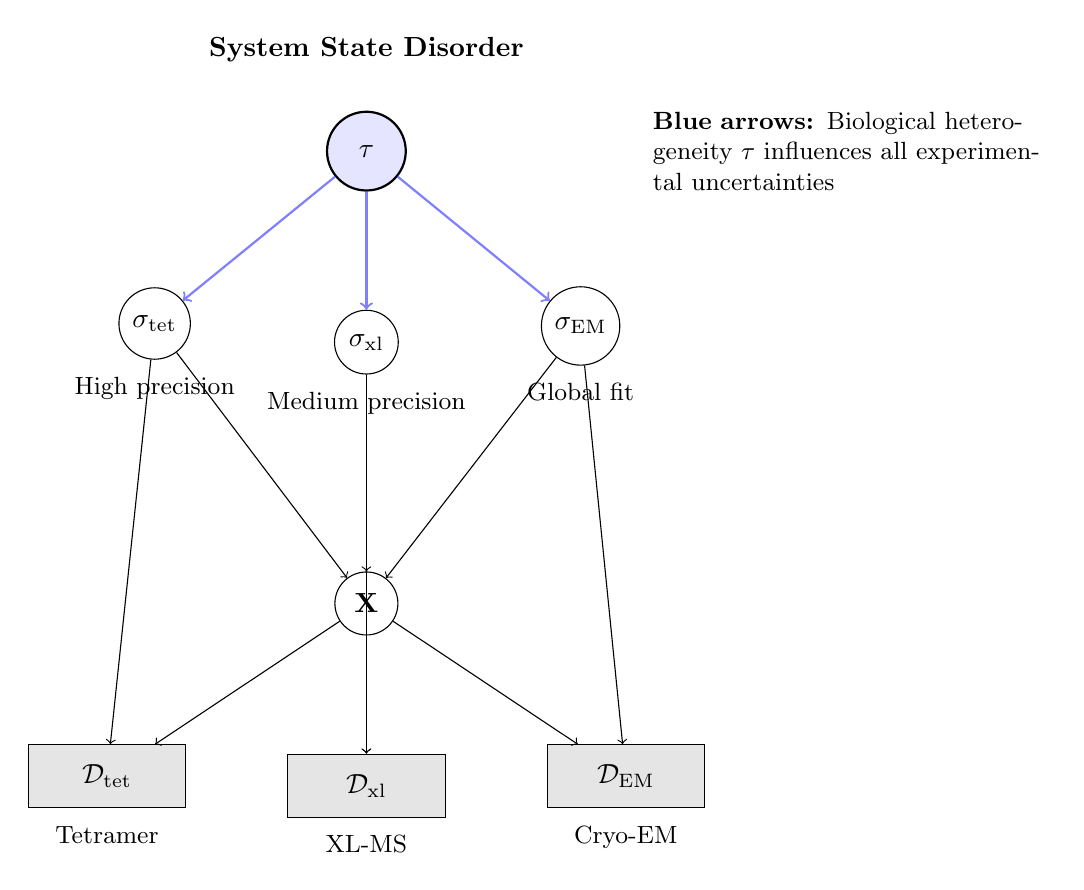
\begin{tikzpicture}[
    node distance=1.5cm,
    box/.style={rectangle, draw, minimum width=2cm, minimum height=0.8cm},
    param/.style={circle, draw, minimum size=0.8cm},
    data/.style={rectangle, draw, fill=gray!20, minimum width=2cm, minimum height=0.8cm},
    hyper/.style={circle, draw, fill=blue!10, minimum size=1cm, thick}
]

% Hyperparameters
\node[hyper] (tau) {$\tau$};
\node[above=0.5cm of tau] {\textbf{System State Disorder}};

% Nuisance parameters
\node[param, below left=1.5cm and 2cm of tau] (sig_tet) {$\sigma_{\text{tet}}$};
\node[param, below=1.5cm of tau] (sig_xl) {$\sigma_{\text{xl}}$};
\node[param, below right=1.5cm and 2cm of tau] (sig_em) {$\sigma_{\text{EM}}$};

% Labels for sigmas
\node[below=0.1cm of sig_tet, font=\small] {High precision};
\node[below=0.1cm of sig_xl, font=\small] {Medium precision};
\node[below=0.1cm of sig_em, font=\small] {Global fit};

% Coordinates
\node[param, below=2.5cm of sig_xl] (X) {$\bX$};

% Data
\node[data, below left=1.5cm and 2cm of X] (D_tet) {$\mathcal{D}_{\text{tet}}$};
\node[data, below=1.5cm of X] (D_xl) {$\mathcal{D}_{\text{xl}}$};
\node[data, below right=1.5cm and 2cm of X] (D_em) {$\mathcal{D}_{\text{EM}}$};

% Data labels
\node[below=0.1cm of D_tet, font=\small] {Tetramer};
\node[below=0.1cm of D_xl, font=\small] {XL-MS};
\node[below=0.1cm of D_em, font=\small] {Cryo-EM};

% Arrows from tau
\draw[->, thick, blue!50] (tau) -- (sig_tet);
\draw[->, thick, blue!50] (tau) -- (sig_xl);
\draw[->, thick, blue!50] (tau) -- (sig_em);

% Arrows to X (implicit via likelihood)
\draw[->] (sig_tet) -- (X);
\draw[->] (sig_xl) -- (X);
\draw[->] (sig_em) -- (X);

% Arrows to data
\draw[->] (X) -- (D_tet);
\draw[->] (X) -- (D_xl);
\draw[->] (X) -- (D_em);
\draw[->] (sig_tet) -- (D_tet);
\draw[->] (sig_xl) -- (D_xl);
\draw[->] (sig_em) -- (D_em);

% Annotation
\node[right=3cm of tau, text width=5cm, font=\small] {
\textbf{Blue arrows:} Biological heterogeneity $\tau$ influences all experimental uncertainties
};

\end{tikzpicture}
\end{center}

\subsection{Prior Distributions}

\subsubsection{Hyperprior on System State Disorder}

The hyperparameter $\tau > 0$ represents the overall degree of biological heterogeneity:
\begin{equation}
    \tau \sim \GammaDist(\alpha_0, \beta_0)
\end{equation}

Typical values: $\alpha_0 = 2$, $\beta_0 = 1$ (weakly informative, allowing $\tau$ to be learned from data).

\textbf{Interpretation:}
\begin{itemize}
    \item $\E[\tau] = \alpha_0 / \beta_0 = 2$: Prior expectation of moderate heterogeneity
    \item $\Var[\tau] = \alpha_0 / \beta_0^2 = 2$: Substantial prior uncertainty
\end{itemize}

\subsubsection{Priors on Nuisance Parameters}

Each nuisance parameter has a prior that depends on $\tau$, with level-specific scaling:

\textbf{Tetramer precision (tight):}
\begin{equation}
    \sigma_{\text{tet}} \sim \HalfCauchy(\tau)
\end{equation}

\textbf{XL-MS precision (looser):}
\begin{equation}
    \sigma_{\text{xl}} \sim \HalfCauchy(\kappa_{\text{xl}} \cdot \tau), \quad \kappa_{\text{xl}} > 1
\end{equation}

\textbf{EM precision:}
\begin{equation}
    \sigma_{\text{EM}} \sim \HalfCauchy(\kappa_{\text{EM}} \cdot \tau)
\end{equation}

The scaling factors $\kappa_{\text{xl}}$ and $\kappa_{\text{EM}}$ encode our prior belief about relative precision:
\begin{itemize}
    \item $\kappa_{\text{xl}} = 3$: XL-MS is expected to be $\sim 3\times$ less precise than tetramer data
    \item $\kappa_{\text{EM}} = 5$: EM fit quality is more uncertain
\end{itemize}

\begin{remark}[Decomposing Uncertainty]
Each $\sigma$ can be conceptually decomposed as:
\begin{equation}
    \sigma_{\text{exp}}^2 = \sigma_{\text{instrumental}}^2 + \sigma_{\text{biological}}^2
\end{equation}
The hierarchical prior, conditioned on $\tau$, primarily captures the $\sigma_{\text{biological}}$ component. The scaling factors $\kappa$ account for different sensitivities of each experiment to biological heterogeneity.
\end{remark}

\subsubsection{Prior on Coordinates}

We use a uniform prior within a bounding box:
\begin{equation}
    p(\bX) = \begin{cases}
        \text{const} & \text{if } \bx_i \in [-L, L]^3 \text{ for all } i \\
        0 & \text{otherwise}
    \end{cases}
\end{equation}

Additional priors can encode:
\begin{itemize}
    \item Excluded volume (no particle overlap)
    \item Connectivity constraints
    \item Symmetry
\end{itemize}

% ===========================================================================
\section{The Full Posterior}
% ===========================================================================

\subsection{Joint Posterior Distribution}

The full posterior over all unknowns is:
\begin{equation}
\boxed{
\begin{aligned}
    p(\bX, \sigma_{\text{tet}}, \sigma_{\text{xl}}, \sigma_{\text{EM}}, \tau \mid \mathcal{D}) 
    &\propto 
    \underbrace{p(\mathcal{D}_{\text{tet}} \mid \bX, \sigma_{\text{tet}})}_{\text{Tetramer likelihood}}
    \cdot \underbrace{p(\mathcal{D}_{\text{xl}} \mid \bX, \sigma_{\text{xl}})}_{\text{XL-MS likelihood}}
    \cdot \underbrace{p(\mathcal{D}_{\text{EM}} \mid \bX, \sigma_{\text{EM}})}_{\text{EM likelihood}} \\
    &\quad \times 
    \underbrace{p(\sigma_{\text{tet}} \mid \tau)}_{\text{Prior}}
    \cdot \underbrace{p(\sigma_{\text{xl}} \mid \tau)}_{\text{Prior}}
    \cdot \underbrace{p(\sigma_{\text{EM}} \mid \tau)}_{\text{Prior}}
    \cdot \underbrace{p(\tau)}_{\text{Hyperprior}}
    \cdot \underbrace{p(\bX)}_{\text{Coord prior}}
\end{aligned}
}
\end{equation}

\subsection{Log-Posterior (for computation)}

For numerical computation, we work with the log-posterior:
\begin{equation}
\begin{aligned}
    \log p(\btheta \mid \mathcal{D}) &= 
    \underbrace{-\frac{1}{2\sigma_{\text{tet}}^2} \sum_{\text{tet pairs}} (d_{ij}^{\text{tet}} - \|\bx_i - \bx_j\|)^2}_{\text{Tetramer log-lik}} \\
    &\quad + \underbrace{-\frac{1}{2\sigma_{\text{xl}}^2} \sum_{\text{XL pairs}} (d_{ij}^{\text{xl}} - \|\bx_i - \bx_j\|)^2}_{\text{XL-MS log-lik}} \\
    &\quad + \underbrace{\frac{\text{CCC}(\bX)}{\sigma_{\text{EM}}^2}}_{\text{EM log-lik}} \\
    &\quad + \underbrace{\log p(\sigma_{\text{tet}} \mid \tau) + \log p(\sigma_{\text{xl}} \mid \tau) + \log p(\sigma_{\text{EM}} \mid \tau)}_{\text{Priors on } \sigma} \\
    &\quad + \underbrace{\log p(\tau)}_{\text{Hyperprior}} + \underbrace{\log p(\bX)}_{\text{Coord prior}} + \text{const}
\end{aligned}
\end{equation}

where $\btheta = (\bX, \sigma_{\text{tet}}, \sigma_{\text{xl}}, \sigma_{\text{EM}}, \tau)$ is the full parameter vector.

% ===========================================================================
\section{Sequential Monte Carlo Sampling}
% ===========================================================================

\subsection{Why SMC?}

The posterior is:
\begin{itemize}
    \item \textbf{High-dimensional}: $3N + 4$ parameters (e.g., $3 \times 32 + 4 = 100$)
    \item \textbf{Multi-modal}: Multiple valid structural configurations
    \item \textbf{Rugged}: Excluded volume creates hard constraints
\end{itemize}

Standard MCMC (e.g., Metropolis-Hastings) struggles with multi-modality. SMC overcomes this by:
\begin{enumerate}
    \item Starting from an easy-to-sample prior
    \item Gradually introducing the likelihood through \textit{tempering}
    \item Maintaining a population of particles that explore different modes
\end{enumerate}

For heterogeneous systems, SMC has an additional advantage: the particle population naturally represents the \textit{ensemble} of structures consistent with the data. Different particles may occupy different modes, collectively capturing the conformational heterogeneity.

\subsection{Tempered SMC Algorithm}

We define a sequence of tempered distributions:
\begin{equation}
    \pi_t(\btheta) \propto p(\btheta) \cdot p(\mathcal{D} \mid \btheta)^{\lambda_t}
\end{equation}

where $0 = \lambda_0 < \lambda_1 < \cdots < \lambda_T = 1$ is the tempering schedule.

\begin{algorithm}[H]
\caption{Adaptive Tempered SMC}
\begin{algorithmic}[1]
\State \textbf{Initialize:} Sample $\{\btheta^{(i)}\}_{i=1}^{M}$ from prior $p(\btheta)$
\State Set $\lambda_0 = 0$, $t = 0$
\While{$\lambda_t < 1$}
    \State \textbf{Adapt $\lambda$:} Find $\lambda_{t+1}$ such that $\text{ESS} = M/2$
    \State \textbf{Reweight:} $w^{(i)} \propto p(\mathcal{D} \mid \btheta^{(i)})^{\lambda_{t+1} - \lambda_t}$
    \State \textbf{Resample:} if ESS too low, resample according to weights
    \State \textbf{Move:} Apply MCMC kernel targeting $\pi_{t+1}$ to each particle
    \State $t \gets t + 1$
\EndWhile
\State \textbf{Return:} Weighted samples $\{(\btheta^{(i)}, w^{(i)})\}_{i=1}^{M}$
\end{algorithmic}
\end{algorithm}

\subsection{MCMC Kernel for Hierarchical Parameters}

Within each SMC step, we use Random Walk Metropolis-Hastings (RMH) with \textbf{different proposal scales} for different parameter types:

\begin{center}
\begin{tabular}{lcc}
\toprule
\textbf{Parameter} & \textbf{Dimension} & \textbf{Proposal $\sigma$} \\
\midrule
Coordinates $\bX$ & $3N$ & 2.0 \AA \\
$\sigma_{\text{tet}}$ & 1 & 0.1 \AA \\
$\sigma_{\text{xl}}$ & 1 & 0.5 \AA \\
$\sigma_{\text{EM}}$ & 1 & 0.2 \\
$\tau$ & 1 & 0.3 \\
\bottomrule
\end{tabular}
\end{center}

This ensures efficient exploration of both coordinate space and nuisance parameter space.

% ===========================================================================
\section{Implementation in JAX}
% ===========================================================================

\subsection{State Vector}

We concatenate all parameters into a single vector for BlackJAX:
\begin{equation}
    \btheta = [\underbrace{x_1, y_1, z_1, \ldots, x_N, y_N, z_N}_{3N \text{ coordinates}}, 
               \underbrace{\sigma_{\text{tet}}, \sigma_{\text{xl}}, \sigma_{\text{EM}}, \tau}_{4 \text{ nuisance params}}]
\end{equation}

\subsection{Code Structure}

\begin{verbatim}
def unpack_state(state):
    """Split state into coordinates and nuisance parameters."""
    coords = state[:-4].reshape(-1, 3)
    sigma_tet = state[-4]
    sigma_xl = state[-3]
    sigma_em = state[-2]
    tau = state[-1]
    return coords, sigma_tet, sigma_xl, sigma_em, tau

def log_prior_fn(state):
    coords, sigma_tet, sigma_xl, sigma_em, tau = unpack_state(state)
    
    # Coordinate prior (in box)
    logp = log_box_prior(coords)
    
    # Hyperprior on tau (System State Disorder)
    logp += gamma_logpdf(tau, alpha=2.0, beta=1.0)
    
    # Priors on sigmas (half-Cauchy, conditioned on tau)
    logp += half_cauchy_logpdf(sigma_tet, scale=tau)
    logp += half_cauchy_logpdf(sigma_xl, scale=3.0 * tau)
    logp += half_cauchy_logpdf(sigma_em, scale=5.0 * tau)
    
    return logp

def log_likelihood_fn(state):
    coords, sigma_tet, sigma_xl, sigma_em, tau = unpack_state(state)
    
    # Level 1: Tetramer distances
    loglik = tetramer_log_likelihood(coords, sigma_tet)
    
    # Level 2: XL-MS distances
    loglik += xlms_log_likelihood(coords, sigma_xl)
    
    # Level 3: EM density
    loglik += em_log_likelihood(coords, sigma_em)
    
    return loglik

def log_prob_fn(state):
    return log_prior_fn(state) + log_likelihood_fn(state)
\end{verbatim}

% ===========================================================================
\section{Interpretation and Diagnostics}
% ===========================================================================

\subsection{Posterior Inference on Nuisance Parameters}

After SMC sampling, we obtain posterior distributions for all nuisance parameters:
\begin{itemize}
    \item $p(\sigma_{\text{tet}} \mid \mathcal{D})$: Inferred precision of tetramer measurements
    \item $p(\sigma_{\text{xl}} \mid \mathcal{D})$: Inferred precision of XL-MS
    \item $p(\sigma_{\text{EM}} \mid \mathcal{D})$: Inferred weight of EM data
    \item $p(\tau \mid \mathcal{D})$: Overall system state disorder
\end{itemize}

\textbf{Key insight:} If $\sigma_{\text{xl}}$ is inferred to be large, the model is ``learning'' that XL-MS data is noisy and should be down-weighted.

\subsection{Interpreting the Hyperparameter $\tau$}

The posterior on $\tau$ provides a direct readout of biological heterogeneity:

\begin{center}
\begin{tabular}{ll}
\toprule
\textbf{Posterior on $\tau$} & \textbf{Biological Interpretation} \\
\midrule
$\tau$ small, tight distribution & Rigid, well-defined structure \\
$\tau$ large, tight distribution & Consistently heterogeneous system \\
$\tau$ has wide distribution & Uncertainty about heterogeneity level \\
\bottomrule
\end{tabular}
\end{center}

\subsection{Distinguishing Noise from Heterogeneity}

The hierarchical structure allows us to distinguish two scenarios:

\textbf{Scenario 1: One noisy experiment}
\begin{itemize}
    \item $\sigma_{\text{xl}}$ is large, but $\sigma_{\text{tet}}$ and $\sigma_{\text{EM}}$ are small
    \item $\tau$ remains small
    \item Interpretation: XL-MS has instrumental problems; other data are reliable
\end{itemize}

\textbf{Scenario 2: Biological heterogeneity}
\begin{itemize}
    \item All $\sigma$ values are elevated (relative to prior expectations)
    \item $\tau$ is large
    \item Interpretation: The system is genuinely heterogeneous; all experiments reflect this
\end{itemize}

\subsection{Model Comparison}

The SMC normalizing constant estimate:
\begin{equation}
    \hat{Z} = \prod_{t=1}^{T} \left( \frac{1}{M} \sum_{i=1}^{M} w_t^{(i)} \right)
\end{equation}
provides an estimate of the marginal likelihood $p(\mathcal{D})$, useful for:
\begin{itemize}
    \item Comparing different hierarchical structures
    \item Model selection (e.g., should EM and XL-MS share a hyperparameter?)
    \item Evaluating whether a heterogeneity model is warranted
\end{itemize}

\subsection{Diagnostics}

\begin{itemize}
    \item \textbf{ESS over tempering steps:} Should not drop too rapidly
    \item \textbf{Acceptance rates:} Target 20-40\% for RMH
    \item \textbf{Posterior predictive checks:} Simulate data from posterior and compare to observed
    \item \textbf{Trace plots:} Visualize parameter evolution across SMC steps
    \item \textbf{$\tau$ vs.\ $\sigma$ correlations:} Check that hierarchical structure is appropriate
\end{itemize}

% ===========================================================================
\section{Summary and Extensions}
% ===========================================================================

\subsection{Key Takeaways}

\begin{enumerate}
    \item \textbf{Noise is signal:} For heterogeneous systems, experimental ``inconsistencies'' contain information about biological variability, not just instrumental error.
    
    \item \textbf{Hierarchical modeling} connects nuisance parameters across data sources through a shared hyperparameter $\tau$ representing system state disorder.
    
    \item \textbf{Different precision levels} are encoded through scaling factors ($\kappa$) in the prior, reflecting our expectations about each experiment's sensitivity to heterogeneity.
    
    \item \textbf{SMC sampling} handles multi-modality, provides normalizing constant estimates, and naturally represents conformational ensembles.
    
    \item \textbf{Automatic calibration}: The posterior on $\sigma$ values learns appropriate data weights; the posterior on $\tau$ quantifies overall heterogeneity.
\end{enumerate}

\subsection{Extensions}

\begin{itemize}
    \item \textbf{Per-restraint nuisance parameters:} $\sigma_{ij}$ for each distance restraint, with a shared prior
    \item \textbf{Outlier modeling:} Mixture models for false positive cross-links
    \item \textbf{Rigid body representation:} Reduce DOF by treating tetramers as rigid units
    \item \textbf{Multiple conformations:} Explicit mixture of structures to model discrete heterogeneity
    \item \textbf{Hierarchical copy numbers:} Treat stoichiometry as a latent variable
\end{itemize}

\subsection{Graphical Model Summary}

The complete model in plate notation:

\begin{center}
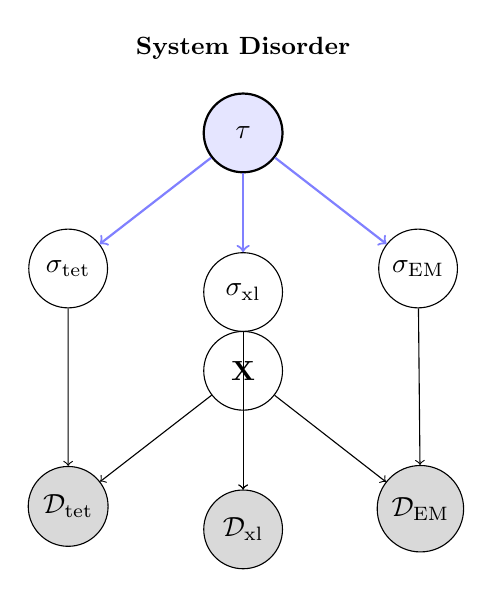
\begin{tikzpicture}[
    node distance=1.2cm,
    obs/.style={circle, draw, fill=gray!30, minimum size=1cm},
    latent/.style={circle, draw, minimum size=1cm},
    hyper/.style={circle, draw, fill=blue!10, minimum size=1cm, thick},
    plate/.style={rectangle, draw, dashed, inner sep=10pt}
]

% Hyperparameter
\node[hyper] (tau) {$\tau$};
\node[above=0.3cm of tau, font=\small\bfseries] {System Disorder};

% Nuisance parameters
\node[latent, below left=1cm and 1.5cm of tau] (s1) {$\sigma_{\text{tet}}$};
\node[latent, below=1cm of tau] (s2) {$\sigma_{\text{xl}}$};
\node[latent, below right=1cm and 1.5cm of tau] (s3) {$\sigma_{\text{EM}}$};

% Coordinates
\node[latent, below=2cm of tau] (X) {$\bX$};

% Observations
\node[obs, below left=1cm and 1.5cm of X] (d1) {$\mathcal{D}_{\text{tet}}$};
\node[obs, below=1cm of X] (d2) {$\mathcal{D}_{\text{xl}}$};
\node[obs, below right=1cm and 1.5cm of X] (d3) {$\mathcal{D}_{\text{EM}}$};

% Arrows
\draw[->, blue!50, thick] (tau) -- (s1);
\draw[->, blue!50, thick] (tau) -- (s2);
\draw[->, blue!50, thick] (tau) -- (s3);
\draw[->] (s1) -- (d1);
\draw[->] (s2) -- (d2);
\draw[->] (s3) -- (d3);
\draw[->] (X) -- (d1);
\draw[->] (X) -- (d2);
\draw[->] (X) -- (d3);

\end{tikzpicture}
\end{center}

% ===========================================================================
\appendix
\section{Probability Distributions}
% ===========================================================================

\subsection{Half-Cauchy Distribution}

The Half-Cauchy distribution with scale $s$ has density:
\begin{equation}
    p(x \mid s) = \frac{2}{\pi s} \cdot \frac{1}{1 + (x/s)^2}, \quad x > 0
\end{equation}

Log-density:
\begin{equation}
    \log p(x \mid s) = \log 2 - \log \pi - \log s - \log\left(1 + (x/s)^2\right)
\end{equation}

\subsection{Gamma Distribution}

The Gamma distribution with shape $\alpha$ and rate $\beta$:
\begin{equation}
    p(x \mid \alpha, \beta) = \frac{\beta^\alpha}{\Gamma(\alpha)} x^{\alpha-1} e^{-\beta x}, \quad x > 0
\end{equation}

\subsection{Inverse-Gamma Distribution}

For variance parameters, the Inverse-Gamma is often used:
\begin{equation}
    p(\sigma^2 \mid \alpha, \beta) = \frac{\beta^\alpha}{\Gamma(\alpha)} (\sigma^2)^{-\alpha-1} \exp\left(-\frac{\beta}{\sigma^2}\right)
\end{equation}

\end{document}